\documentclass[a4paper, 14pt]{extarticle}
\usepackage{float}
% Поля
%--------------------------------------
\usepackage{geometry}
\geometry{a4paper,tmargin=2cm,bmargin=2cm,lmargin=3cm,rmargin=1cm}
%--------------------------------------


%Russian-specific packages
%--------------------------------------
\usepackage[T2A]{fontenc}
\usepackage[utf8]{inputenc}
\usepackage[english, main=russian]{babel}
%--------------------------------------

\usepackage{textcomp}

% Красная строка
%--------------------------------------
\usepackage{indentfirst}
%--------------------------------------


%Graphics
%--------------------------------------
\usepackage{graphicx}
\graphicspath{ {./images/} }
\usepackage{wrapfig}
%--------------------------------------

% Полуторный интервал
%--------------------------------------
\linespread{1.3}
%--------------------------------------

%Выравнивание и переносы
%--------------------------------------
% Избавляемся от переполнений
\sloppy
% Запрещаем разрыв страницы после первой строки абзаца
\clubpenalty=10000
% Запрещаем разрыв страницы после последней строки абзаца
\widowpenalty=10000
%--------------------------------------

%Списки
\usepackage{enumitem}

%Подписи
\usepackage{caption}

%Гиперссылки
\usepackage{hyperref}

\usepackage{float}

\hypersetup {
	unicode=true
}

%Рисунки
%--------------------------------------
\DeclareCaptionLabelSeparator*{emdash}{~--- }
\captionsetup[figure]{labelsep=emdash,font=onehalfspacing,position=bottom}
%--------------------------------------

\usepackage{tempora}

%Листинги
%--------------------------------------
\usepackage{listings}
\lstset{
  basicstyle=\ttfamily\footnotesize,
  %basicstyle=\footnotesize\AnkaCoder,        % the size of the fonts that are used for the code
  breakatwhitespace=false,        % sets if automatic breaks shoulbd only happen at whitespace
  breaklines=true,                 % sets automatic line breaking
  captionpos=t,                    % sets the caption-position to bottom
  inputencoding=utf8,
  frame=single,                    % adds a frame around the code
  keepspaces=true,                 % keeps spaces in text, useful for keeping indentation of code (possibly needs columns=flexible)
  keywordstyle=\bf,       % keyword style
  numbers=left,                    % where to put the line-numbers; possible values are (none, left, right)
  numbersep=5pt,                   % how far the line-numbers are from the code
  xleftmargin=25pt,
  xrightmargin=25pt,
  showspaces=false,                % show spaces everywhere adding particular underscores; it overrides 'showstringspaces'
  showstringspaces=false,          % underline spaces within strings only
  showtabs=false,                  % show tabs within strings adding particular underscores
  stepnumber=1,                    % the step between two line-numbers. If it's 1, each line will be numbered
  tabsize=2,                       % sets default tabsize to 8 spaces
  title=\lstname                   % show the filename of files included with \lstinputlisting; also try caption instead of title
}
%--------------------------------------

%%% Математические пакеты %%%
%--------------------------------------
\usepackage{amsthm,amsfonts,amsmath,amssymb,amscd}  % Математические дополнения от AMS
\usepackage{mathtools}                              % Добавляет окружение multlined
\usepackage[perpage]{footmisc}
%--------------------------------------

%--------------------------------------
%			НАЧАЛО ДОКУМЕНТА
%--------------------------------------

\begin{document}

%--------------------------------------
%			ТИТУЛЬНЫЙ ЛИСТ
%--------------------------------------
\begin{titlepage}
\thispagestyle{empty}
\newpage


%Шапка титульного листа
%--------------------------------------
\vspace*{-60pt}
\hspace{-65pt}
\begin{minipage}{0.3\textwidth}
\hspace*{-20pt}\centering

\includegraphics[width=\textwidth]{emblem}
\end{minipage}
\begin{minipage}{0.67\textwidth}\small \textbf{
\vspace*{-0.7ex}
\hspace*{-6pt}\centerline{Министерство науки и высшего образования Российской Федерации}
\vspace*{-0.7ex}
\centerline{Федеральное государственное бюджетное образовательное учреждение }
\vspace*{-0.7ex}
\centerline{высшего образования}
\vspace*{-0.7ex}
\centerline{<<Московский государственный технический университет}
\vspace*{-0.7ex}
\centerline{имени Н.Э. Баумана}
\vspace*{-0.7ex}
\centerline{(национальный исследовательский университет)>>}
\vspace*{-0.7ex}
\centerline{(МГТУ им. Н.Э. Баумана)}}
\end{minipage}
%--------------------------------------

%Полосы
%--------------------------------------
\vspace{-25pt}
\hspace{-35pt}\rule{\textwidth}{2.3pt}

\vspace*{-20.3pt}
\hspace{-35pt}\rule{\textwidth}{0.4pt}
%--------------------------------------

\vspace{1.5ex}
\hspace{-35pt} \noindent \small ФАКУЛЬТЕТ\hspace{80pt} <<Информатика и системы управления>>

\vspace*{-16pt}
\hspace{47pt}\rule{0.83\textwidth}{0.4pt}

\vspace{0.5ex}
\hspace{-35pt} \noindent \small КАФЕДРА\hspace{50pt} <<Теоретическая информатика и компьютерные технологии>>

\vspace*{-16pt}
\hspace{30pt}\rule{0.866\textwidth}{0.4pt}

\vspace{11em}

\begin{center}
\Large {\bf Лабораторная работа № 2} \\
\large {\bf по курсу <<Теория искусственных нейронных сетей>>} \\
\large <<Разработка многослойного персептрона
на основе обратного распространения ошибки FFNN>>
\end{center}\normalsize

\vspace{8em}


\begin{flushright}
  {Студент группы ИУ9-71Б Баев Д.А \hspace*{15pt}\\
  \vspace{2ex}
  Преподаватель Каганов Ю. Т.\hspace*{15pt}}
\end{flushright}

\bigskip

\vfill


\begin{center}
\textsl{Москва 2023}
\end{center}
\end{titlepage}
%--------------------------------------
%		КОНЕЦ ТИТУЛЬНОГО ЛИСТА
%--------------------------------------

\renewcommand{\ttdefault}{pcr}

\setlength{\tabcolsep}{3pt}
\newpage
\setcounter{page}{2}

\section{Задание}\label{Sect::task}
1. Реализовать на языке высокого уровня многослойный персептрон и 
проверить его работоспособность на примере данных, выбранных из 
MNIST dataset. 

2. Исследовать работу персептрона на основе использования различных 
целевых функций. (среднеквадратичная ошибка, перекрестная 
энтропия, дивергенция Кульбака-Лейблера).

3. Исследовать работу многослойного персептрона с использованием 
различных методов оптимизации (градиентный, Флетчера-Ривза (FR), 
Бройдена-Флетчера-Гольдфарба-Шенно (BFGS)).

4. Провести исследование эффективности работы многослойного 
персептрона при изменении гиперпараметров (количества нейронов и 
количества слоев).

5. Подготовить отчет с распечаткой текста программы, графиками 
результатов исследования и анализом результатов.
\newpage
\section{Исходный код}

Исходный код программы представлен в листингах~\ref{lst:code1}-~\ref{lst:code6}

\begin{lstlisting}[language={},caption={Подготовка датасета},label={lst:code1}, breaklines=true]
import numpy as np
import pandas as pd
import matplotlib.pyplot as plt
import torchvision
from tqdm import tqdm

MNIST_train = torchvision.datasets.MNIST('./', download=True, train=True)
MNIST_test = torchvision.datasets.MNIST('./', download=True, train=False)

count = 480
count_test = 80

train_X = MNIST_train.data.numpy()[:count]
train_Y = MNIST_train.targets.numpy()[:count]
test_X = MNIST_test.data.numpy()[:count_test]
test_Y = MNIST_test.targets.numpy()[:count_test]

train_X = np.array(list(map(lambda x: x.flatten() / 256, train_X)))
train_Y = np.array([np.array([int(i == x) for i in range(10)]) for x in train_Y])
test_X = np.array(list(map(lambda x: x.flatten() / 256, test_X)))
test_Y = np.array([np.array([int(i == x) for i in range(10)]) for x in test_Y])
\end{lstlisting}


\begin{lstlisting}[language={},caption={Определение функций активации и функций ошибки},label={lst:code2}, breaklines=true]
def softmax(x):
    if np.linalg.norm(x) < 0.001:
        return np.zeros(len(x))
    x = x / np.linalg.norm(x)
    return np.exp(x)/(np.exp(x)).sum() if (np.exp(x)).sum() > 0.01 else np.zeros(len(x))

def relu(x):
    return np.maximum(0, x)

def relu_derivative(x):
    return np.where(x > 0, 1, 0)

def mse(y_true, y_pred):
    return np.sum((y_true - y_pred) ** 2) / len(y_true)

def mse_derivative(y_true, y_pred):
    return 2 * (y_pred - y_true) / len(y_true)

def sigmoid(x): return 1/(1+np.exp(-x))
def sigmoid_derivative(x): return sigmoid(x)*(1-sigmoid(x))

def cross_entropy(y_true, y_pred):
    y_pred = np.clip(y_pred, 1e-8, 1 - 1e-8)
    return -np.mean(y_true * np.log(y_pred))

def cross_entropy_derivative(y_true, y_pred):
    y_pred = np.clip(y_pred, 1e-8, 1 - 1e-8)
    res = y_pred - y_true
    return res / np.linalg.norm(res)

def kl_divergence(y_true, y_pred):
    y_true = np.clip(y_true, 1e-8, 1- 1e-8)
    y_pred = np.clip(y_pred, 1e-8, 1-1e-8)
    return np.mean(y_true * np.log(y_true / y_pred))

def kl_divergence_derivative(y_true, y_pred):
    y_pred = np.clip(y_pred, 1e-8, 1 - 1e-8)
    res = y_pred - y_true
    return res / np.linalg.norm(res)
\end{lstlisting}




\begin{lstlisting}[language={},caption={Класс линейного слоя},label={lst:code3}, breaklines=true]
class LinearLayer:
    def __init__(self, input_size, output_size, optimizer, model):
        self.hessian = None
        self.previous_weights = None
        self.previous_grad = None
        self.inputs = None
        self.weights = np.random.rand(input_size + 1, output_size) - 0.5
        self.optimizer = optimizer
        self.model = model

    def forward(self, inputs, train=True):
        inputs = np.append([1], inputs)

        if train:
            self.inputs = inputs
        return inputs @ self.weights

    def calculate_forward(self):
        return self.model.calculate_forward(self, self.inputs[1:])

    def backward(self, grad):
        accum_grad = (grad @ self.weights.T)[1:]
        step_grad = np.outer(self.inputs, grad)
        if np.linalg.norm(step_grad) != 0:
            step_grad /= np.linalg.norm(step_grad)
        step = None
        match self.optimizer:
            case 0:
                # GD
                step = step_grad
            case 1:
                # FR
                if self.previous_grad is None:
                    self.previous_grad = step_grad
                    w = 0
                else:
                    grad = step_grad.flatten()
                    previous_grad = self.previous_grad.flatten()
                    w = max((np.linalg.norm(grad)/np.linalg.norm(previous_grad)) ** 2, 0)
                    if np.isnan(w) or w == np.Inf:
                        w = 0
                step = (step_grad + w * self.previous_grad)
                self.previous_grad = step_grad
            case 2:
                # BFGS
                if self.hessian is None:
                    self.hessian = np.identity(len(step_grad))
                    self.previous_grad = np.zeros(step_grad.shape)
                    self.previous_weights = np.zeros(self.weights.shape)

                step = self.hessian @ step_grad

                s = self.weights - self.previous_weights
                y = step_grad - self.previous_grad

                w = np.identity(len(step_grad)) - s @ y.T
                self.hessian = w @ self.hessian @ w.T

                self.previous_grad = step_grad
                self.previous_weights = self.weights


        step *= self.model.lr

        before = self.calculate_forward()
        self.weights -= step
        after = self.calculate_forward()
        if before > after and abs(after - before) > 0.0001:
            while before > after and abs(after - before) > 0.0001:
                self.weights -= step
                before = after
                after = self.calculate_forward()
            self.weights += step
        return accum_grad
\end{lstlisting}


\begin{lstlisting}[language={},caption={Класс слоя активации},label={lst:code4}, breaklines=true]
class ActivationLayer:
    def __init__(self, activation, activation_derivative):
        self.inputs = None
        self.activation = activation
        self.activation_derivative = activation_derivative
    def forward(self, inputs, train=True):
        self.inputs = inputs
        return self.activation(inputs)
    def backward(self, grad):
        return grad * self.activation_derivative(self.inputs)

\end{lstlisting}




\begin{lstlisting}[language={},caption={Класс перцептрона},label={lst:code5}, breaklines=true]
class Perceptron:
    def __init__(self, input_size, sizes, loss, loss_derivative, optimizer, lr):
        self.last_true = None
        self.layers = []
        prev_size = input_size
        for size in sizes:
            self.layers.append(LinearLayer(prev_size, size, optimizer, self))
            self.layers.append(ActivationLayer(sigmoid, sigmoid_derivative))
            prev_size = size
        self.layers.append(LinearLayer(prev_size, 10, optimizer, self))
        self.layers.append(ActivationLayer(softmax, lambda x: softmax(x) * (1 - softmax(x))))
        self.loss = loss
        self.loss_derivative = loss_derivative
        self.lr = lr

    def forward(self, inputs, train=True):
        result = inputs
        for layer in self.layers:
            result = layer.forward(result, train)
        return result

    def backward(self, y_true, y_pred):
        grad = self.loss_derivative(y_true, y_pred)
        for layer in self.layers[::-1]:
            grad = layer.backward(grad)

    def fit(self, inputs, y_true):
        self.last_true = y_true
        y_pred = self.forward(inputs, True)
        loss = self.loss(y_true, y_pred)
        self.backward(y_true, y_pred)
        return y_pred, loss

    def calculate(self, layer, inputs):
        place = self.layers.index(layer)
        result = inputs
        for layer in self.layers[place:]:
            result = layer.forward(result, False)
        return self.loss(self.last_true, result)


    def train(self, epochs):
        accuracy = []
        loss_arr = []
        for _ in tqdm(range(epochs)):
            running_accuracy = 0
            running_loss = 0
            for inputs, y_true in zip(train_X, train_Y):
                y_pred, loss = self.fit(inputs, y_true)
                pred = np.argmax(y_pred)
                running_loss += loss
                running_accuracy += (np.argmax(y_true) == pred)
            accuracy.append(running_accuracy / len(train_X))
            loss_arr.append(running_loss / len(train_X))
        return accuracy, loss_arr

    def validate(self):
        running_accuracy = 0
        running_loss = 0
        for inputs, y_true in zip(test_X, test_Y):
            y_pred = self.forward(inputs, False)
            loss = self.loss(y_true, y_pred)
            pred = np.argmax(y_pred)
            running_loss += loss
            running_accuracy += (np.argmax(y_true) == pred)
        return running_loss / len(test_X), running_accuracy / len(test_X)
\end{lstlisting}


\begin{figure}[H]
\begin{lstlisting}[language={},caption={Класс эксперимента},label={lst:code6}]
def experiment(learning_rate, layer_count, layer_neurons, epochs, optimizer, loss, loss_der):
    perceptron = Perceptron(28 * 28, [layer_neurons for _ in range(layer_count)], loss, loss_der, optimizer, learning_rate)

    accuracy, loss = perceptron.train(epochs)


    plt.plot(np.arange(len(accuracy)), accuracy)
    plt.title("Accuracy")
    plt.show()
    plt.plot(np.arange(len(loss)), loss)
    plt.title("Loss")
    plt.show()

    print(perceptron.validate())
\end{lstlisting}
\end{figure}

\section{Результаты}

В качестве начального эксперимента были выбраны следующие параметры: learning rate - 0.009, количество скрытых слоев (без учета входного и выходного слоев) - 1, количество нейронов в скрытом слое - 64, количество эпох - 40, функция потерь - перекрестная энтропия, оптимизатор - градиентный.

График точности этой модели от количества эпох приведен на рисунке ~\ref{fig:img1}

\begin{figure}[H]
\centering
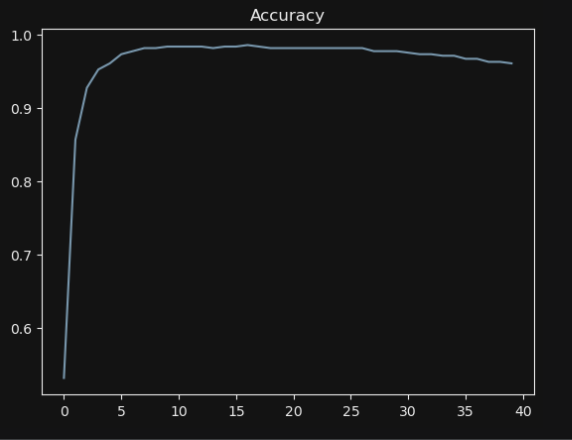
\includegraphics[width=0.8\textwidth]{images/res1.png}
\caption{}
\label{fig:img1}
\end{figure}

Теперь функция потерь изменяется на среднеквадратичную ошибку. График точности измененной модели от количества эпох приведен на рисунке ~\ref{fig:img2}. Видно серьезное ухудшение результата.

\begin{figure}[H]
\centering
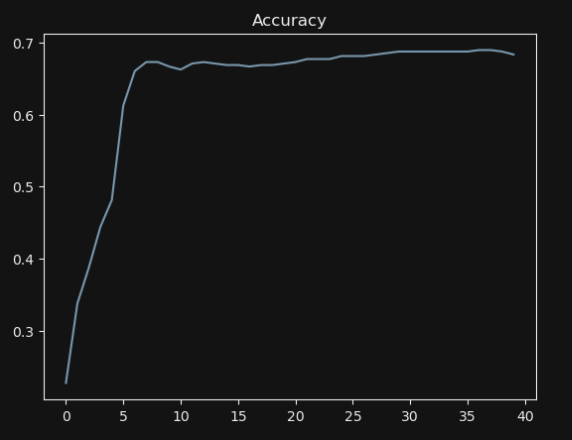
\includegraphics[width=0.8\textwidth]{images/res2.png}
\caption{}
\label{fig:img2}
\end{figure}

Теперь функция потерь изменяется на дивергенцию Кульбака-Лейблера. График точности измененной модели от количества эпох приведен на рисунке ~\ref{fig:img3}. Результат примерно схож с перекрестной энтропией.

\begin{figure}[H]
\centering
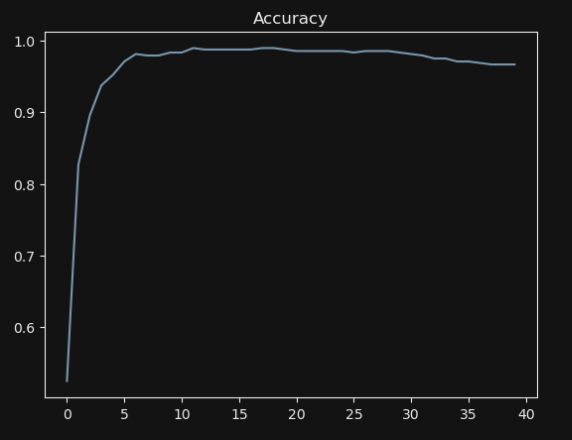
\includegraphics[width=0.8\textwidth]{images/res3.png}
\caption{}
\label{fig:img3}
\end{figure}

Теперь в качестве функции потерь была возвращена перекрестная энтропия. Число скрытых слоев теперь - 0. График точности измененной модели от количества эпох приведен на рисунке ~\ref{fig:img4}. Видно ухудшение результата и расходимость обучения при большем количестве эпох.

\begin{figure}[H]
\centering
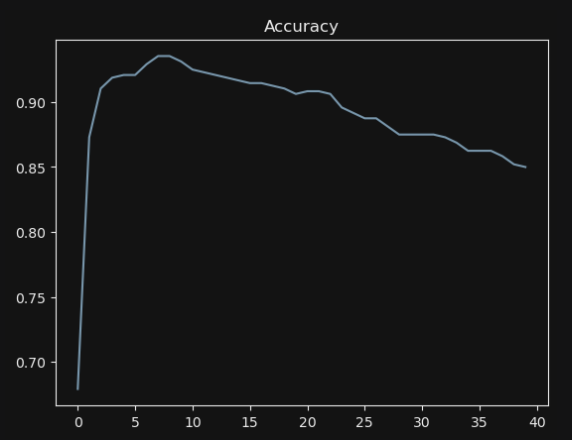
\includegraphics[width=0.8\textwidth]{images/res4.png}
\caption{}
\label{fig:img4}
\end{figure}

Число скрытых слоев теперь - 2. График точности измененной модели от количества эпох приведен на рисунке ~\ref{fig:img5}. Видно ухудшение по сравнению с результатом с одним скрытым слоем. 

\begin{figure}[H]
\centering
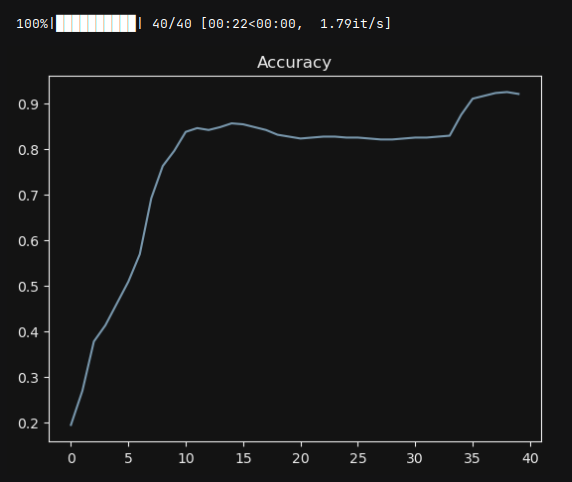
\includegraphics[width=0.8\textwidth]{images/res5.png}
\caption{}
\label{fig:img5}
\end{figure}

Число скрытых слоев теперь - 1. Число нейронов в скрытом слое теперь - 128. График точности измененной модели от количества эпох приведен на рисунке ~\ref{fig:img6}. Результат примерно такой же, как и при 64 нейронах. 

\begin{figure}[H]
\centering
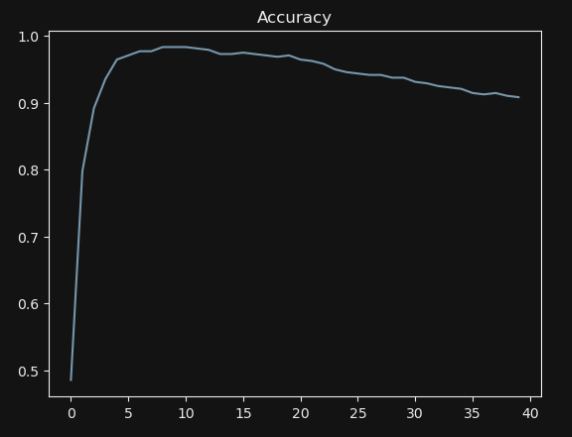
\includegraphics[width=0.8\textwidth]{images/res6.png}
\caption{}
\label{fig:img6}
\end{figure}

Теперь все значения такие же, как и в первом эксперименте. В качестве оптимизатора был выбран FR. График точности измененной модели от количества эпох приведен на рисунке ~\ref{fig:img7}. Видно незначительное ухудшение результата.

\begin{figure}[H]
\centering
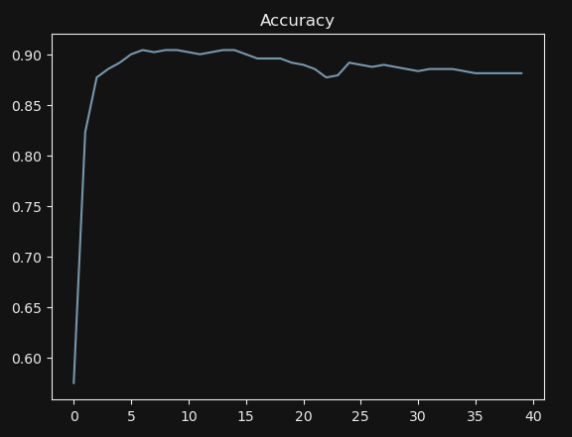
\includegraphics[width=0.8\textwidth]{images/res7.png}
\caption{}
\label{fig:img7}
\end{figure}

Теперь в качестве оптимизатора был выбран BFGS. График точности измененной модели от количества эпох приведен на рисунке ~\ref{fig:img8}. Этот алгоритм оптимизации работает значительно дольше из-за обилия матричных вычислений при расчете Гессиана. Поэтому данная модель обучалась всего 5 эпох. С учетом этого факта, данный алгоритм показал достойный результат.

\begin{figure}[H]
\centering
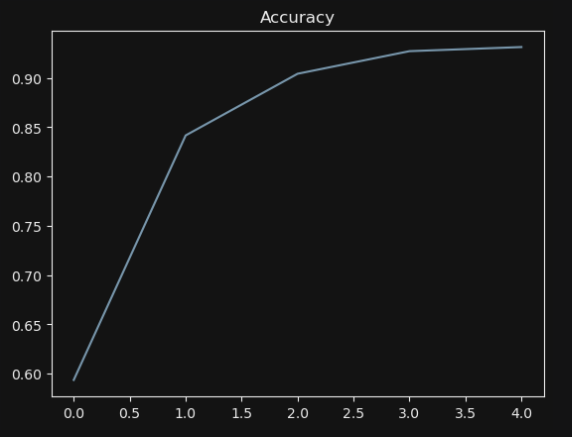
\includegraphics[width=0.8\textwidth]{images/res8.png}
\caption{}
\label{fig:img8}
\end{figure}


В качестве финального эксперимента было проверено повышение количества скрытых слоев (3), чтобы продемонстрировать все большее ухудшение результата. График точности измененной модели от количества эпох приведен на рисунке ~\ref{fig:img9}. 

\begin{figure}[H]
\centering
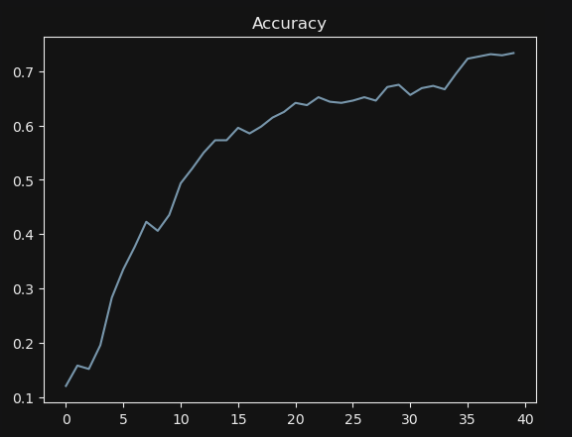
\includegraphics[width=0.8\textwidth]{images/res9.png}
\caption{}
\label{fig:img9}
\end{figure}


\section{Выводы}
В рамках данной лабораторной работы был вручную реализован многослойный перцептрон, решающий задачу классификации рукописных цифр. Были реализованы различные целевые функции: среднеквадратичное отклонение, перекрестная энтропия, дивергенция Кульбака-Лейблера. Были реализованы различные методы оптимизации: градиентный, FR, BFGS. Наилучшие результаты показали перекрестная энтропия и дивергенция Кульбака-Лейбнера в сочетании с одним скрытым слоем и градиентным методом оптимизации. Также хорошо себя зарекомендовал метод BFGS, но в случае его использования происходит большой проигрыш в скорости.
\end{document}
